\chapter{Übertragung}
Bandbreite des Sendesignals:
\[ B \approx \frac{1}{T_S} \]

\begin{center}
	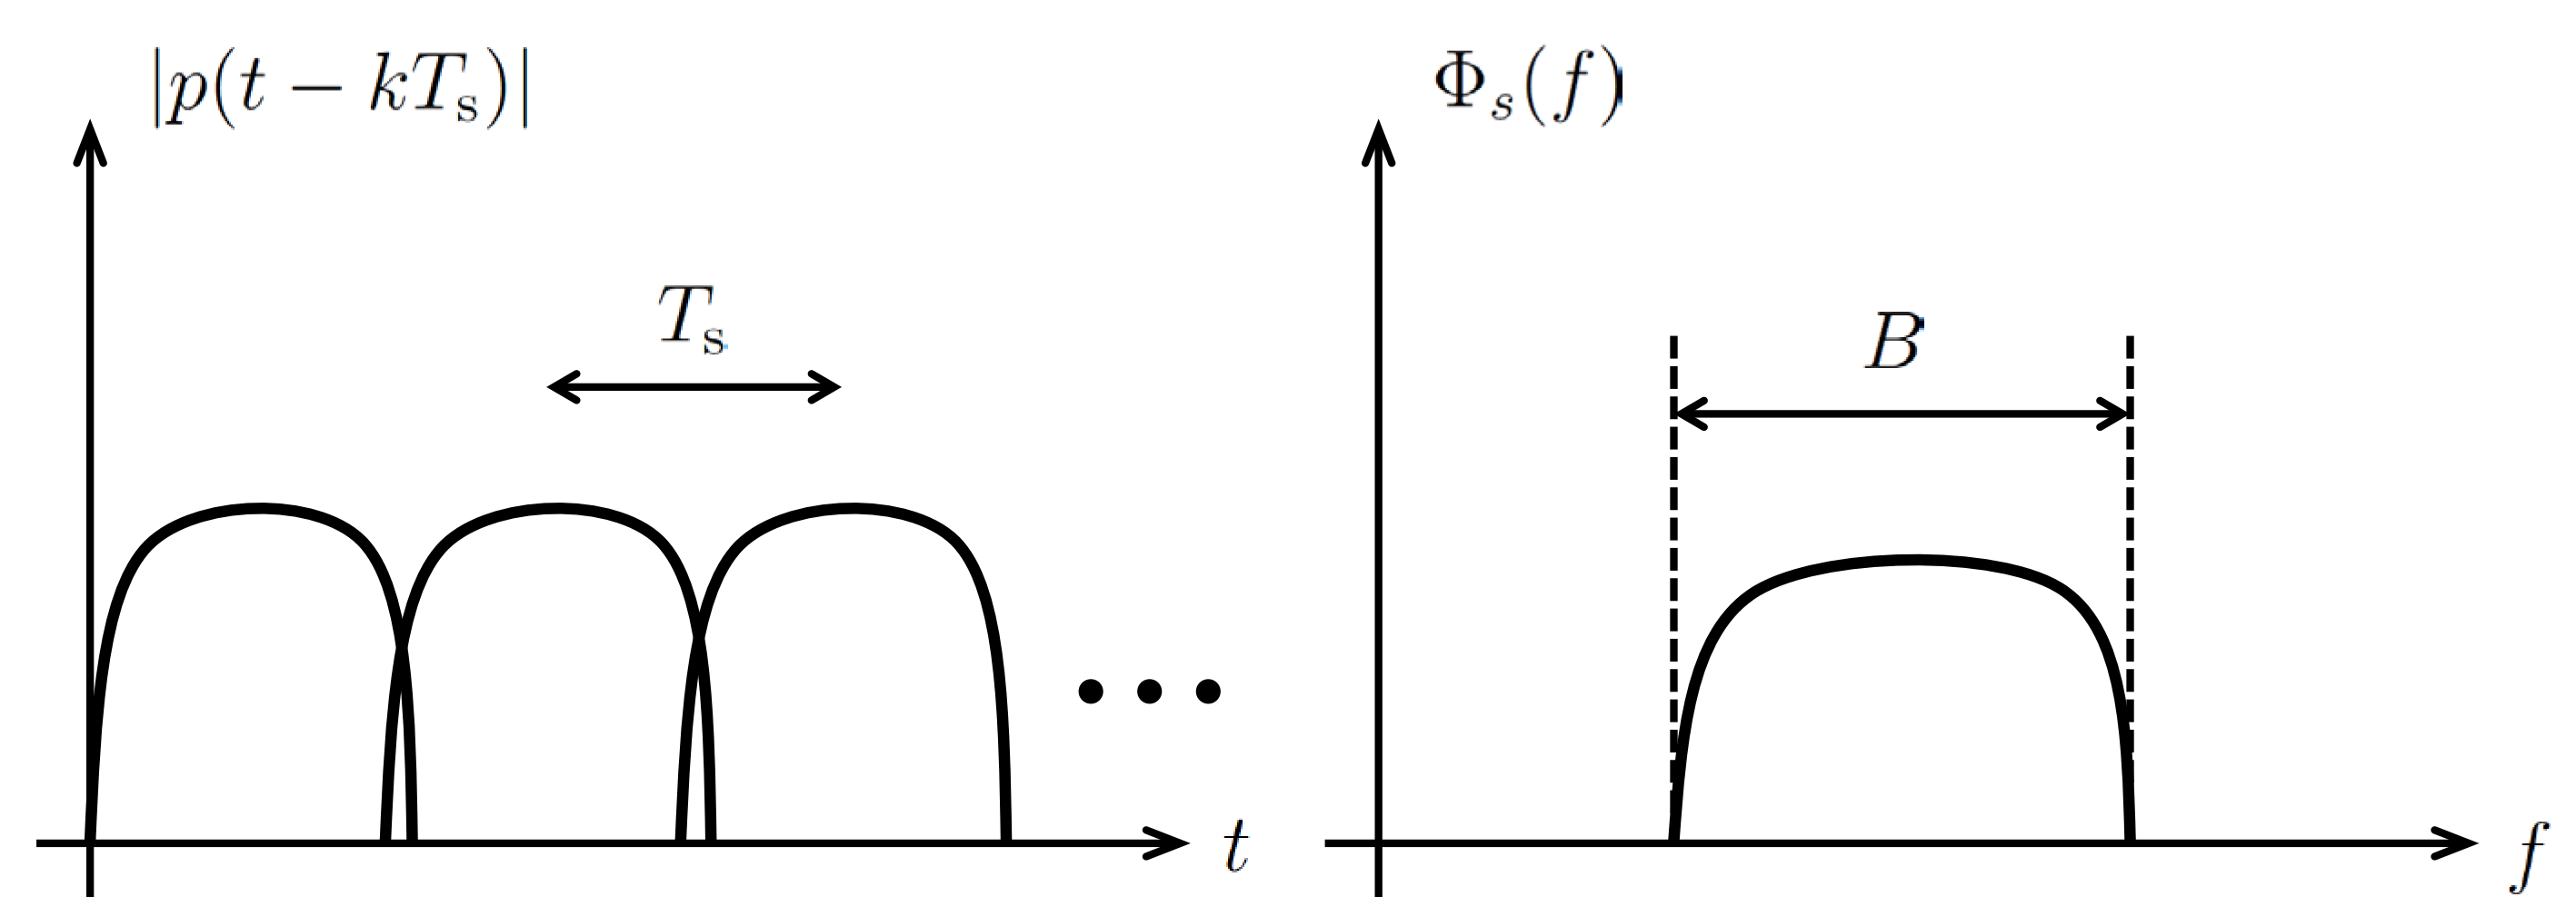
\includegraphics[width=.9\textwidth]{../fig/eintrager.png}
\end{center}

\section{Mehrweg-Ausbreitung}
Kohärenzbandbreite des Kanals:
\[ B_c \approx \frac{1}{\tau_m} \]

\begin{center}
	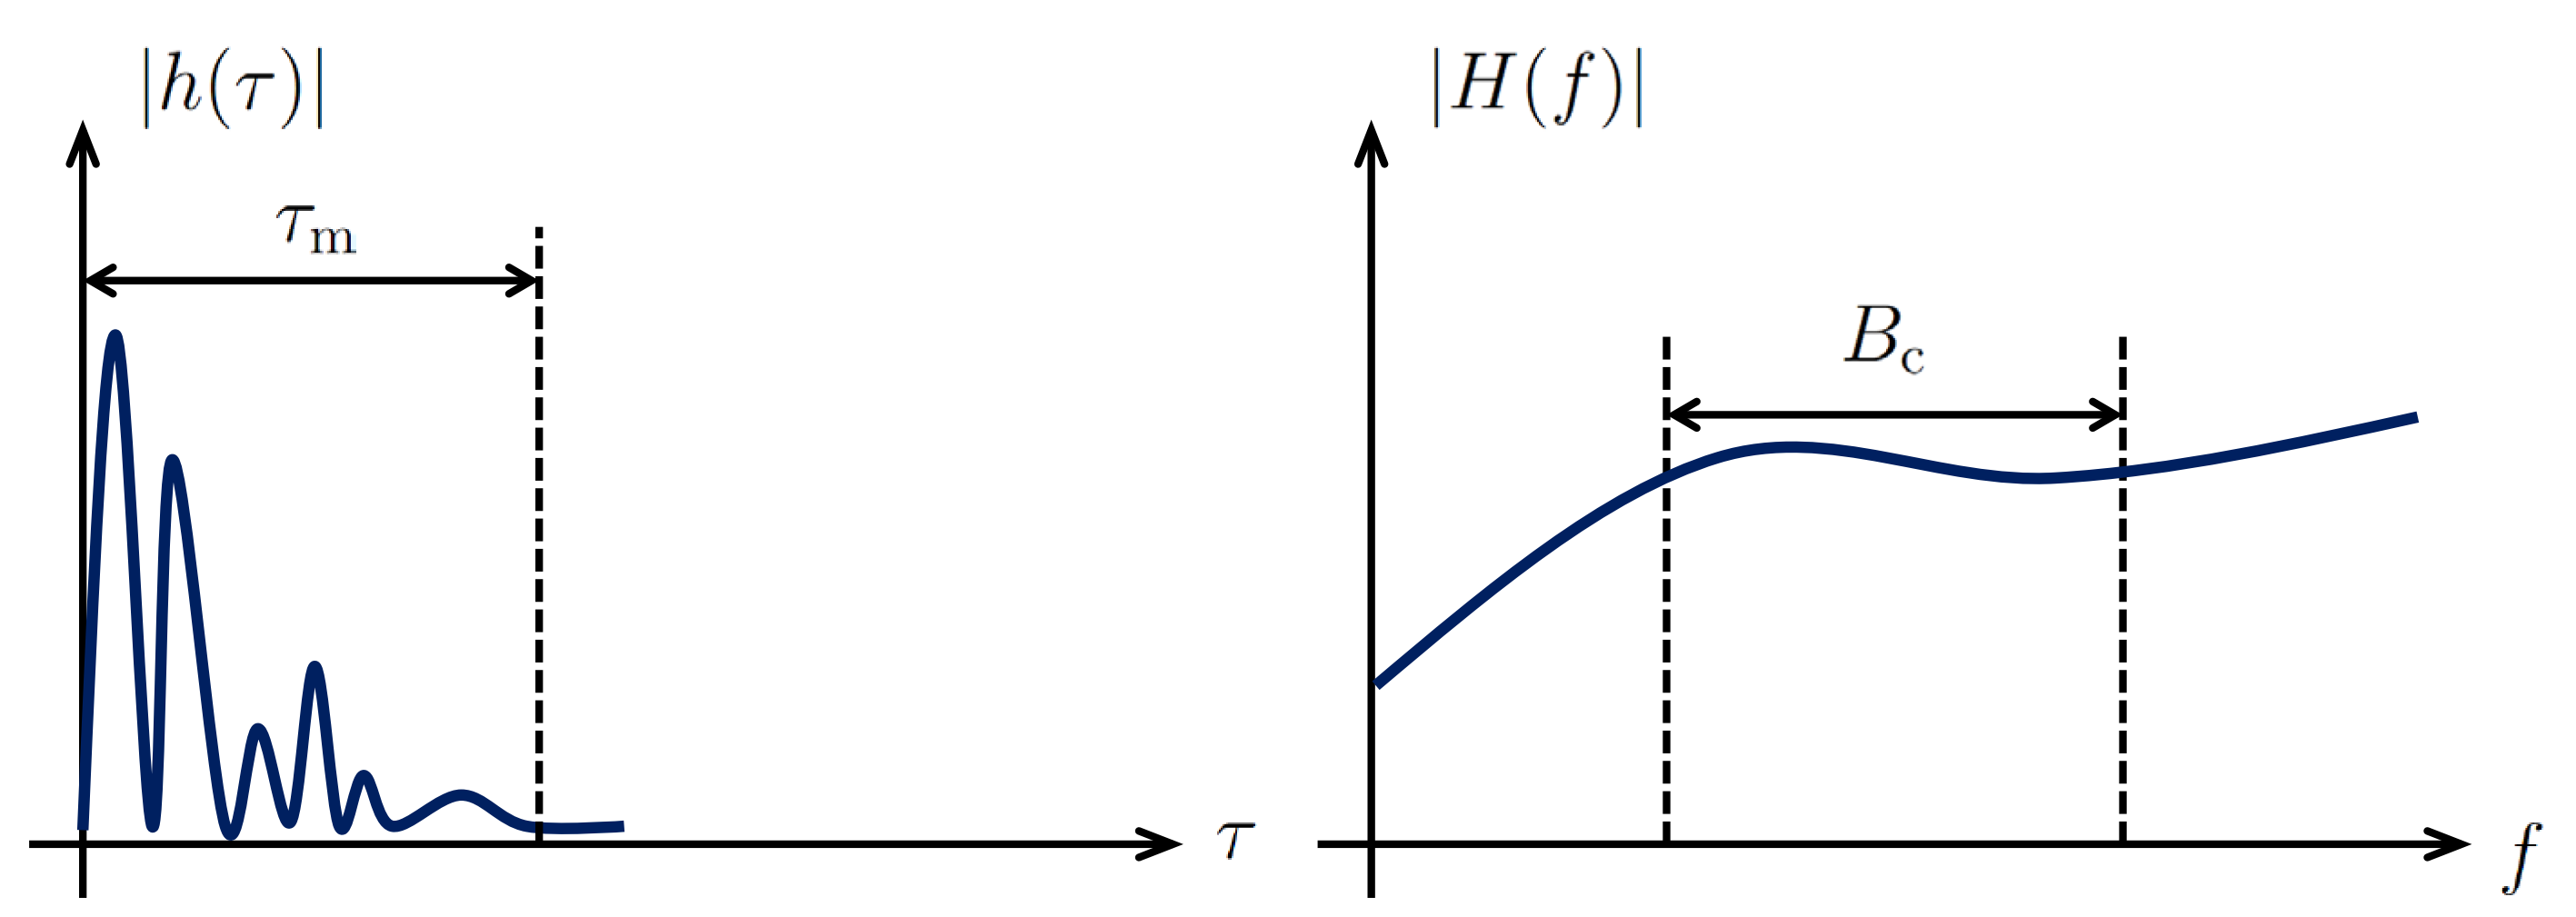
\includegraphics[width=.9\textwidth]{../fig/mehrweg.png}
\end{center}

\section{Verzerrung}
Impuls am Empfänger:
\[ q(t) = (p * h)(t) \]
~\\
Leistungsdichtespektrum des Empfangssignals:
\[ \Phi_r(f) = \Phi_s(f) \cdot |H(f)|^2 \]

\section{Schmalband vs. Breitband}
Symboldauer: $T_s$\\
Bandbreite: $B \approx \frac{1}{T_S}$\\
Multipath Spread: $\tau_m$\\
Kohärenzbandbreite: $B_c \approx \frac{1}{\tau_m}$\\
schmalbandige Übertragung: $\tau_m < T_s$\\
breitbandige Übertragung: $\tau_m > T_s$

\subsection{Schmalbandige Übertragung}
Impuls am Empfänger:
\[ q(t) \approx \alpha \cdot p(t) \]
~\\
Leistungsdichtespektrum des Empfangssignals:
\[ \Phi_r(f) \approx |\alpha|^2 \cdot \Phi_s(f) \]
~\\
\[ \tau_m < T_s \qquad B < B_c \]
\begin{center}
	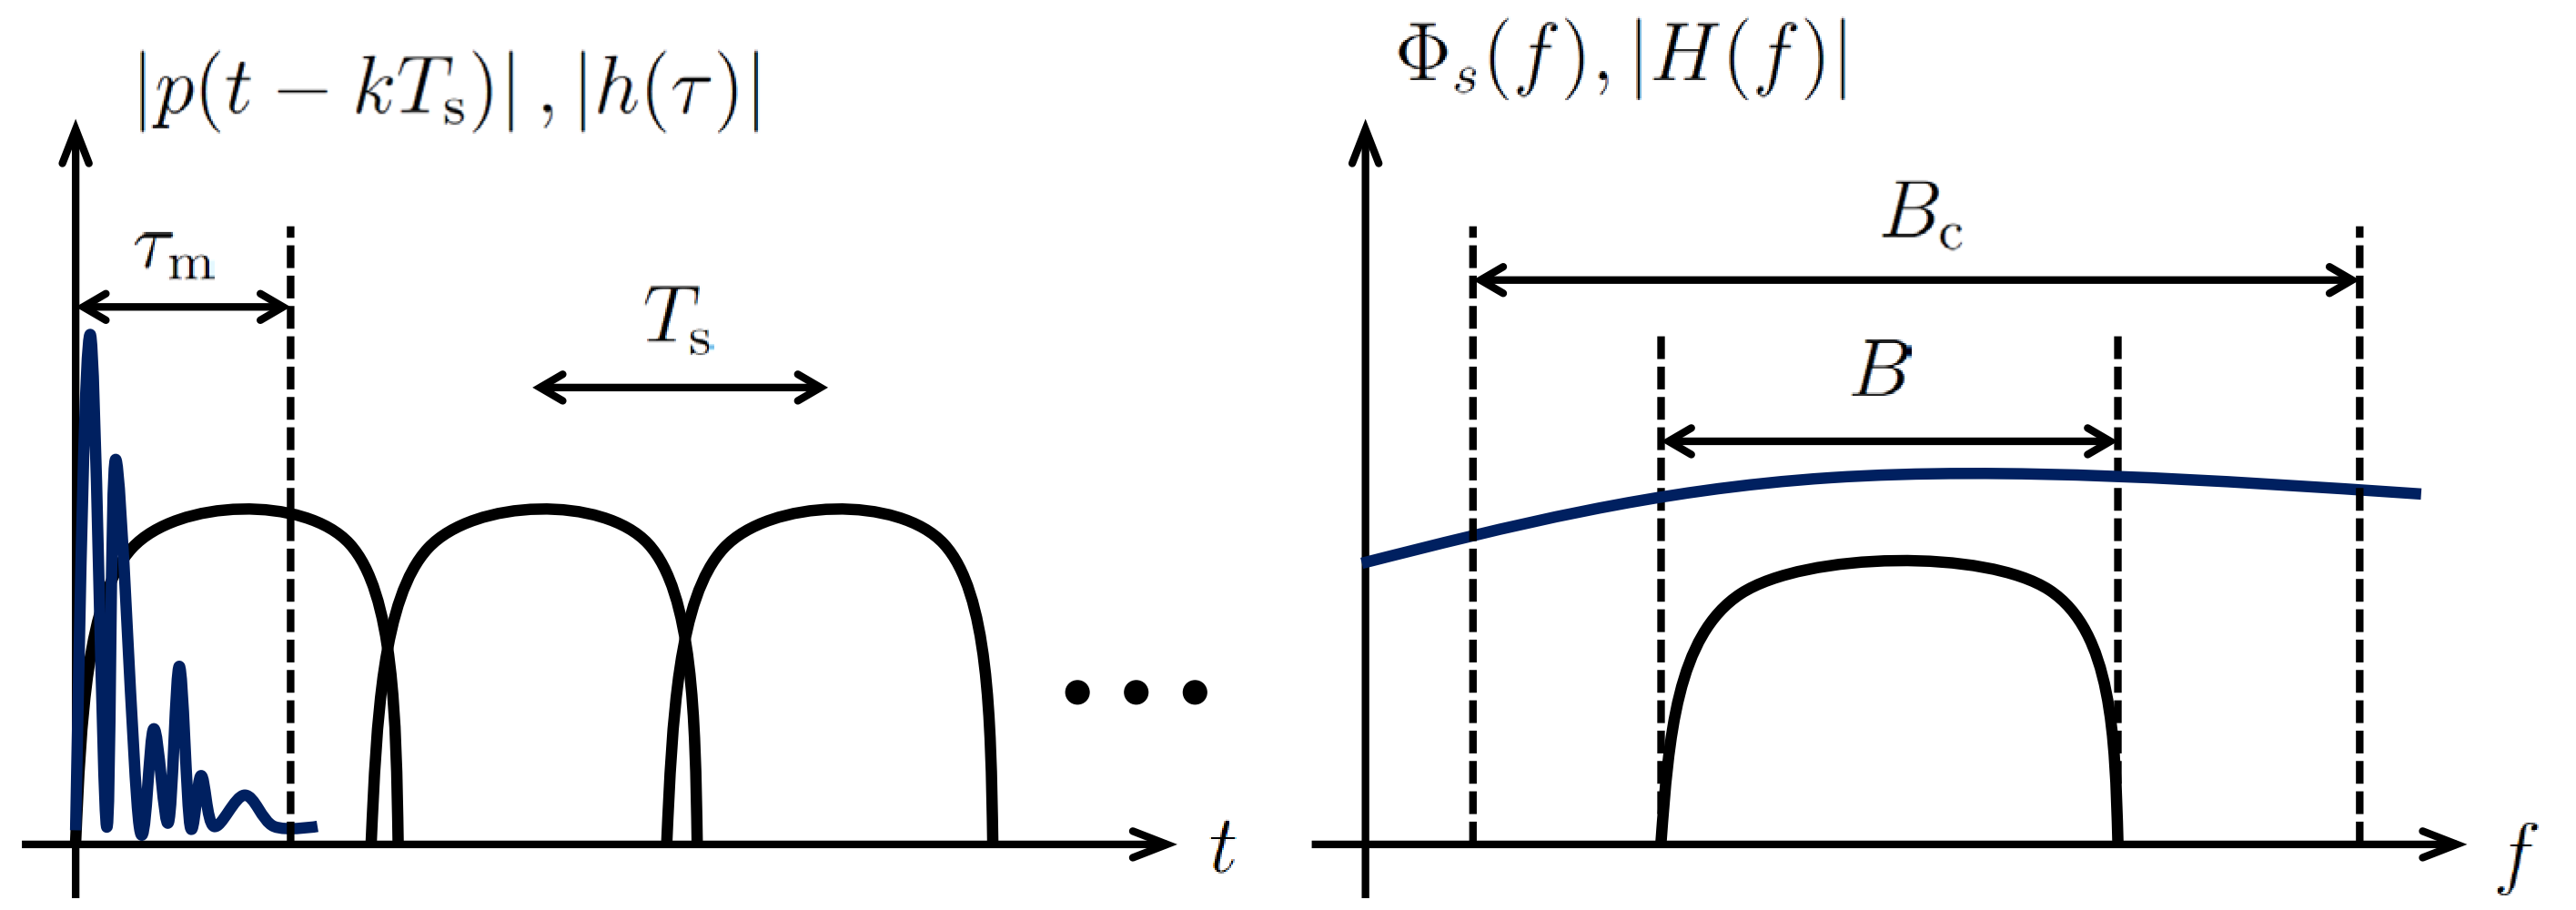
\includegraphics[width=.9\textwidth]{../fig/schmalband.png}
\end{center}
\begin{center}
	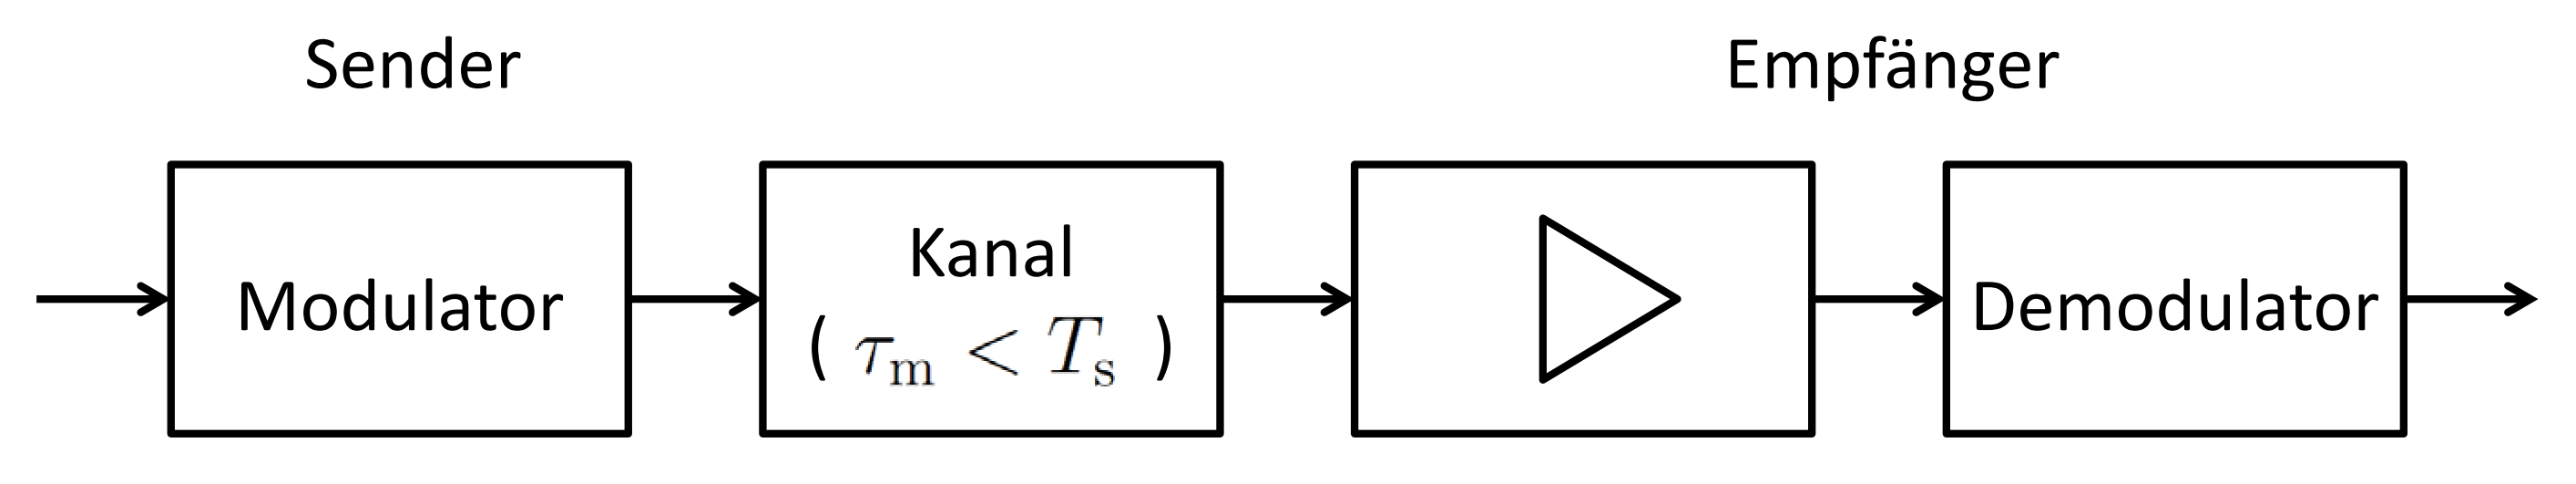
\includegraphics[width=.9\textwidth]{../fig/mod_schmalband.png}
\end{center}

\subsection{Breitbandige Übertragung}
Impuls am Empfänger:
\[ q(t) = (p*h)(t) \]
~\\
Leistungsdichtespektrum des Empfangssignals:
\[ \Phi_r(f) = \Phi_s(f) \cdot |H(f)|^2 \]
~\\
\[ \tau_m > T_s \qquad B > B_c \]
\begin{center}
	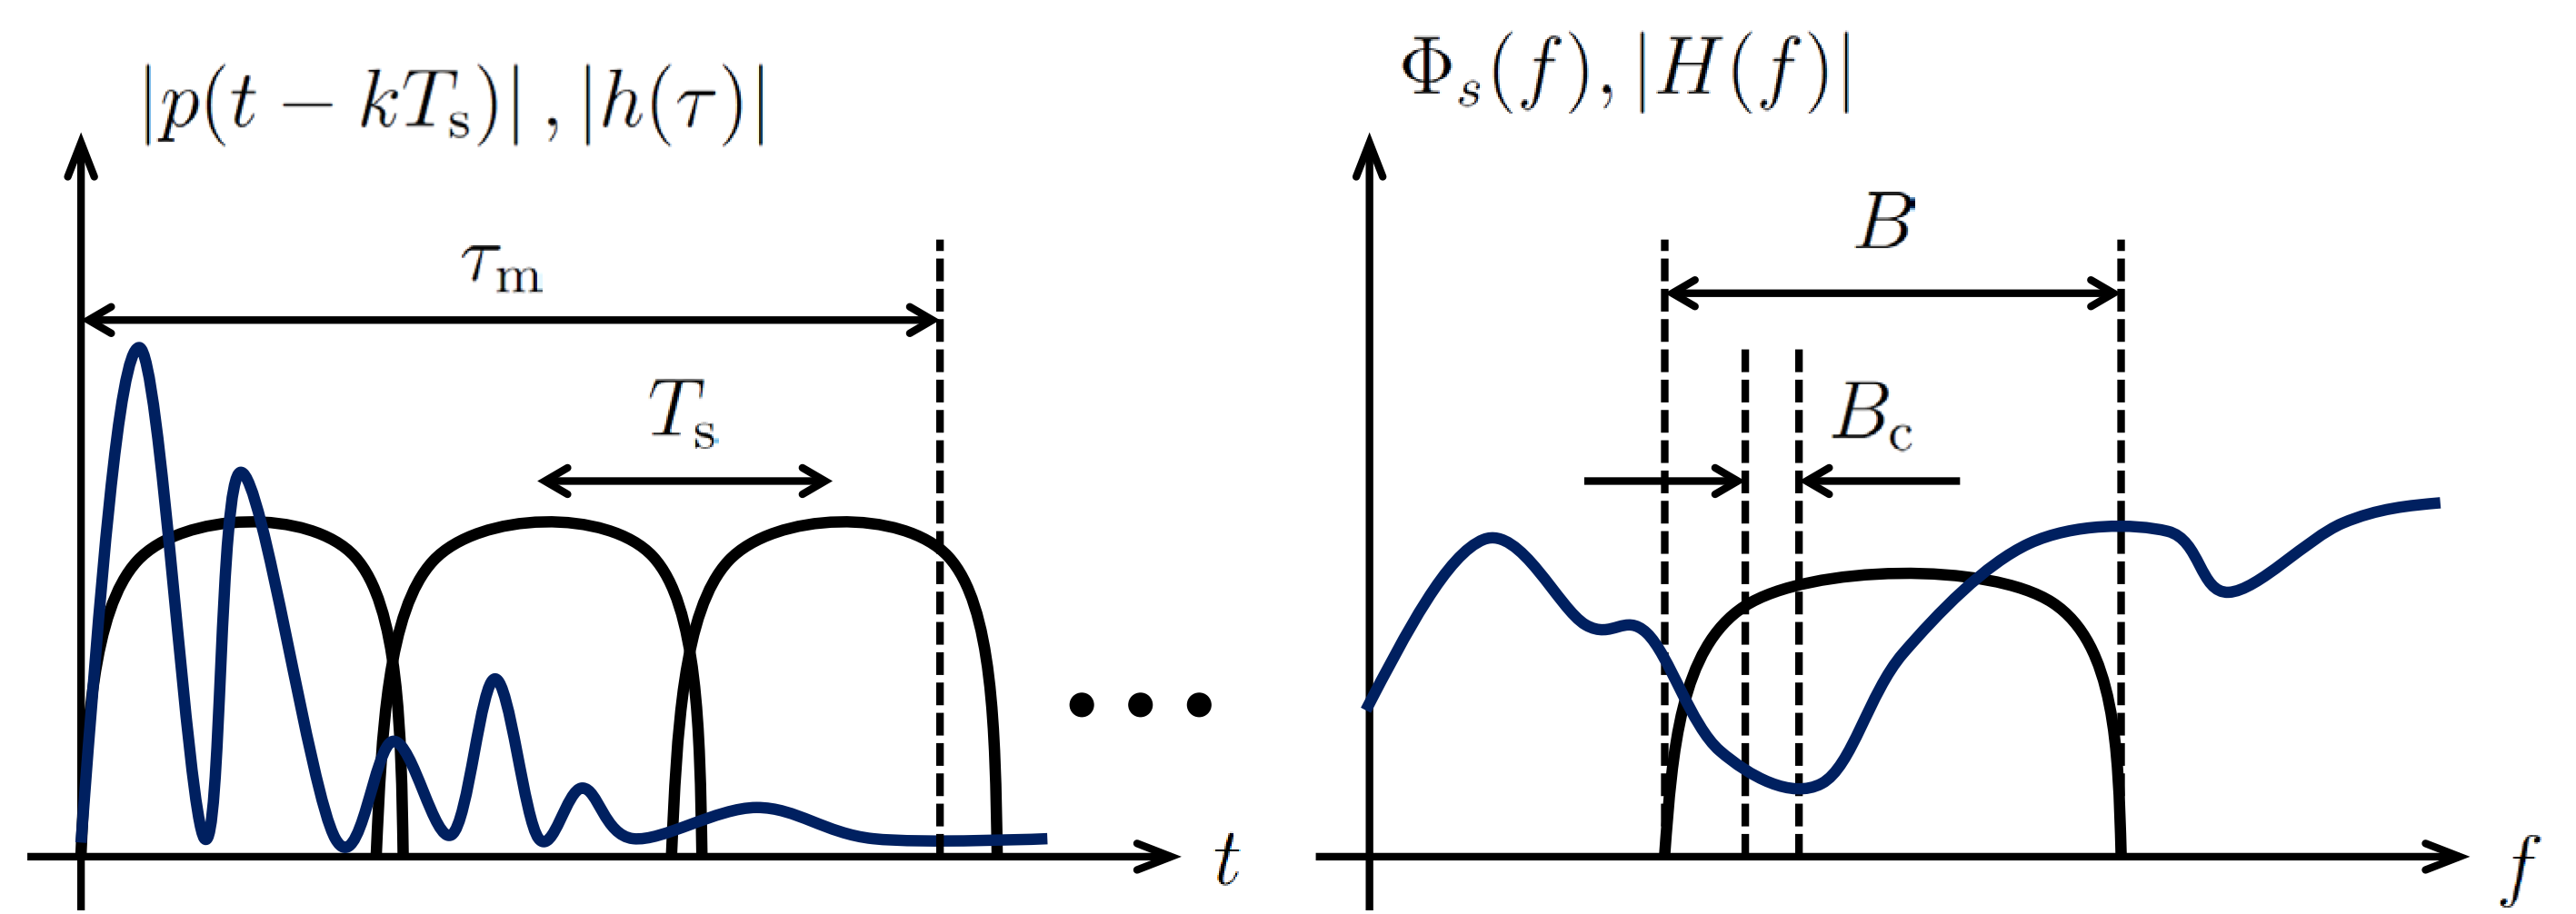
\includegraphics[width=.9\textwidth]{../fig/breitband.png}
\end{center}
\begin{center}
	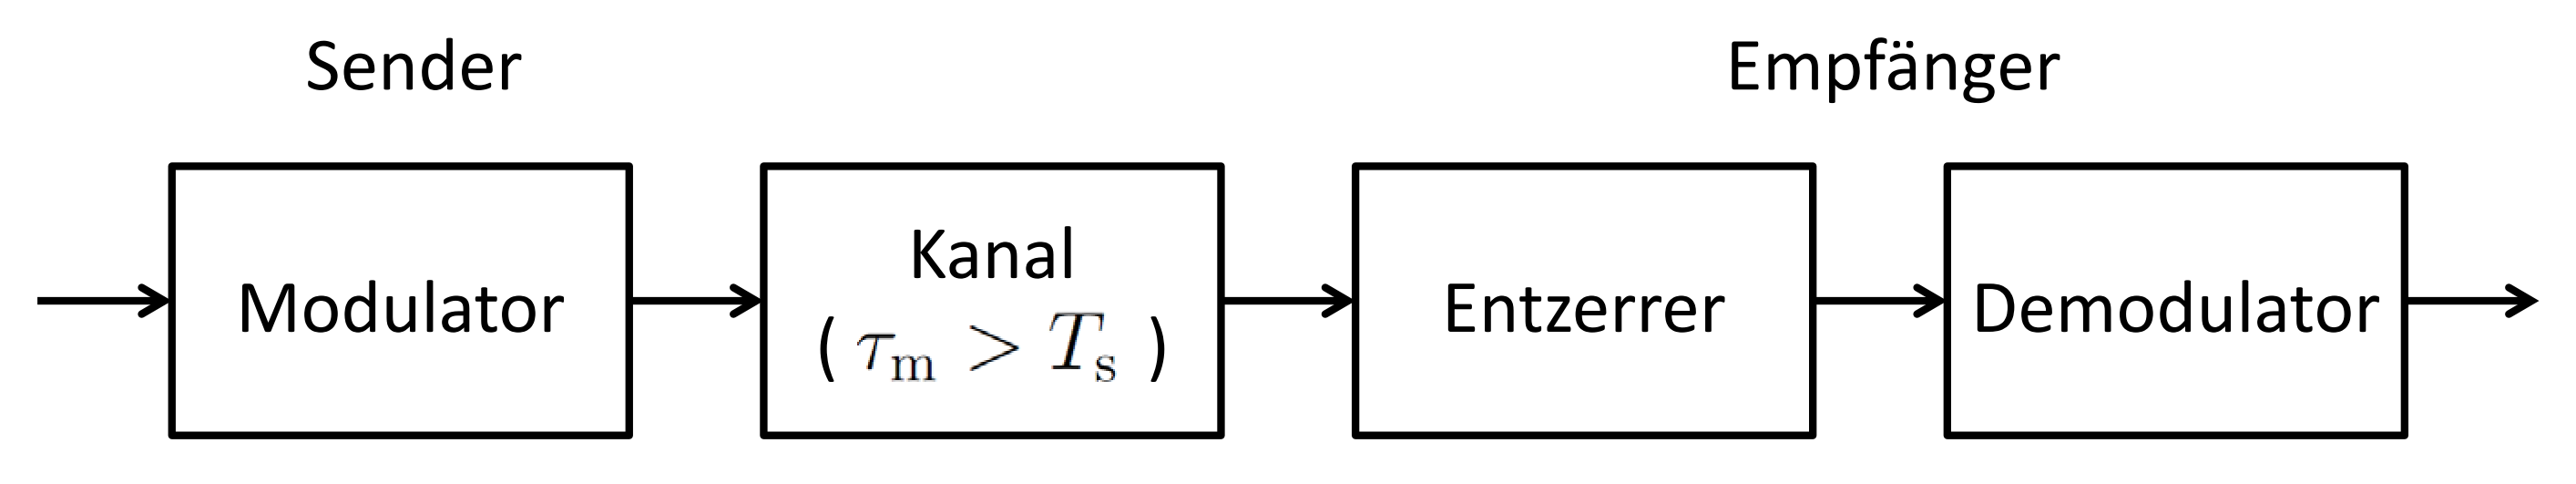
\includegraphics[width=.9\textwidth]{../fig/mod_breitband.png}
\end{center}

\section{Mehrträgerübertragung}
Bandbreite des Sendesignals: $B$\\
Bandbreite eines Unterträgers: $B_{sc}$

\begin{center}
	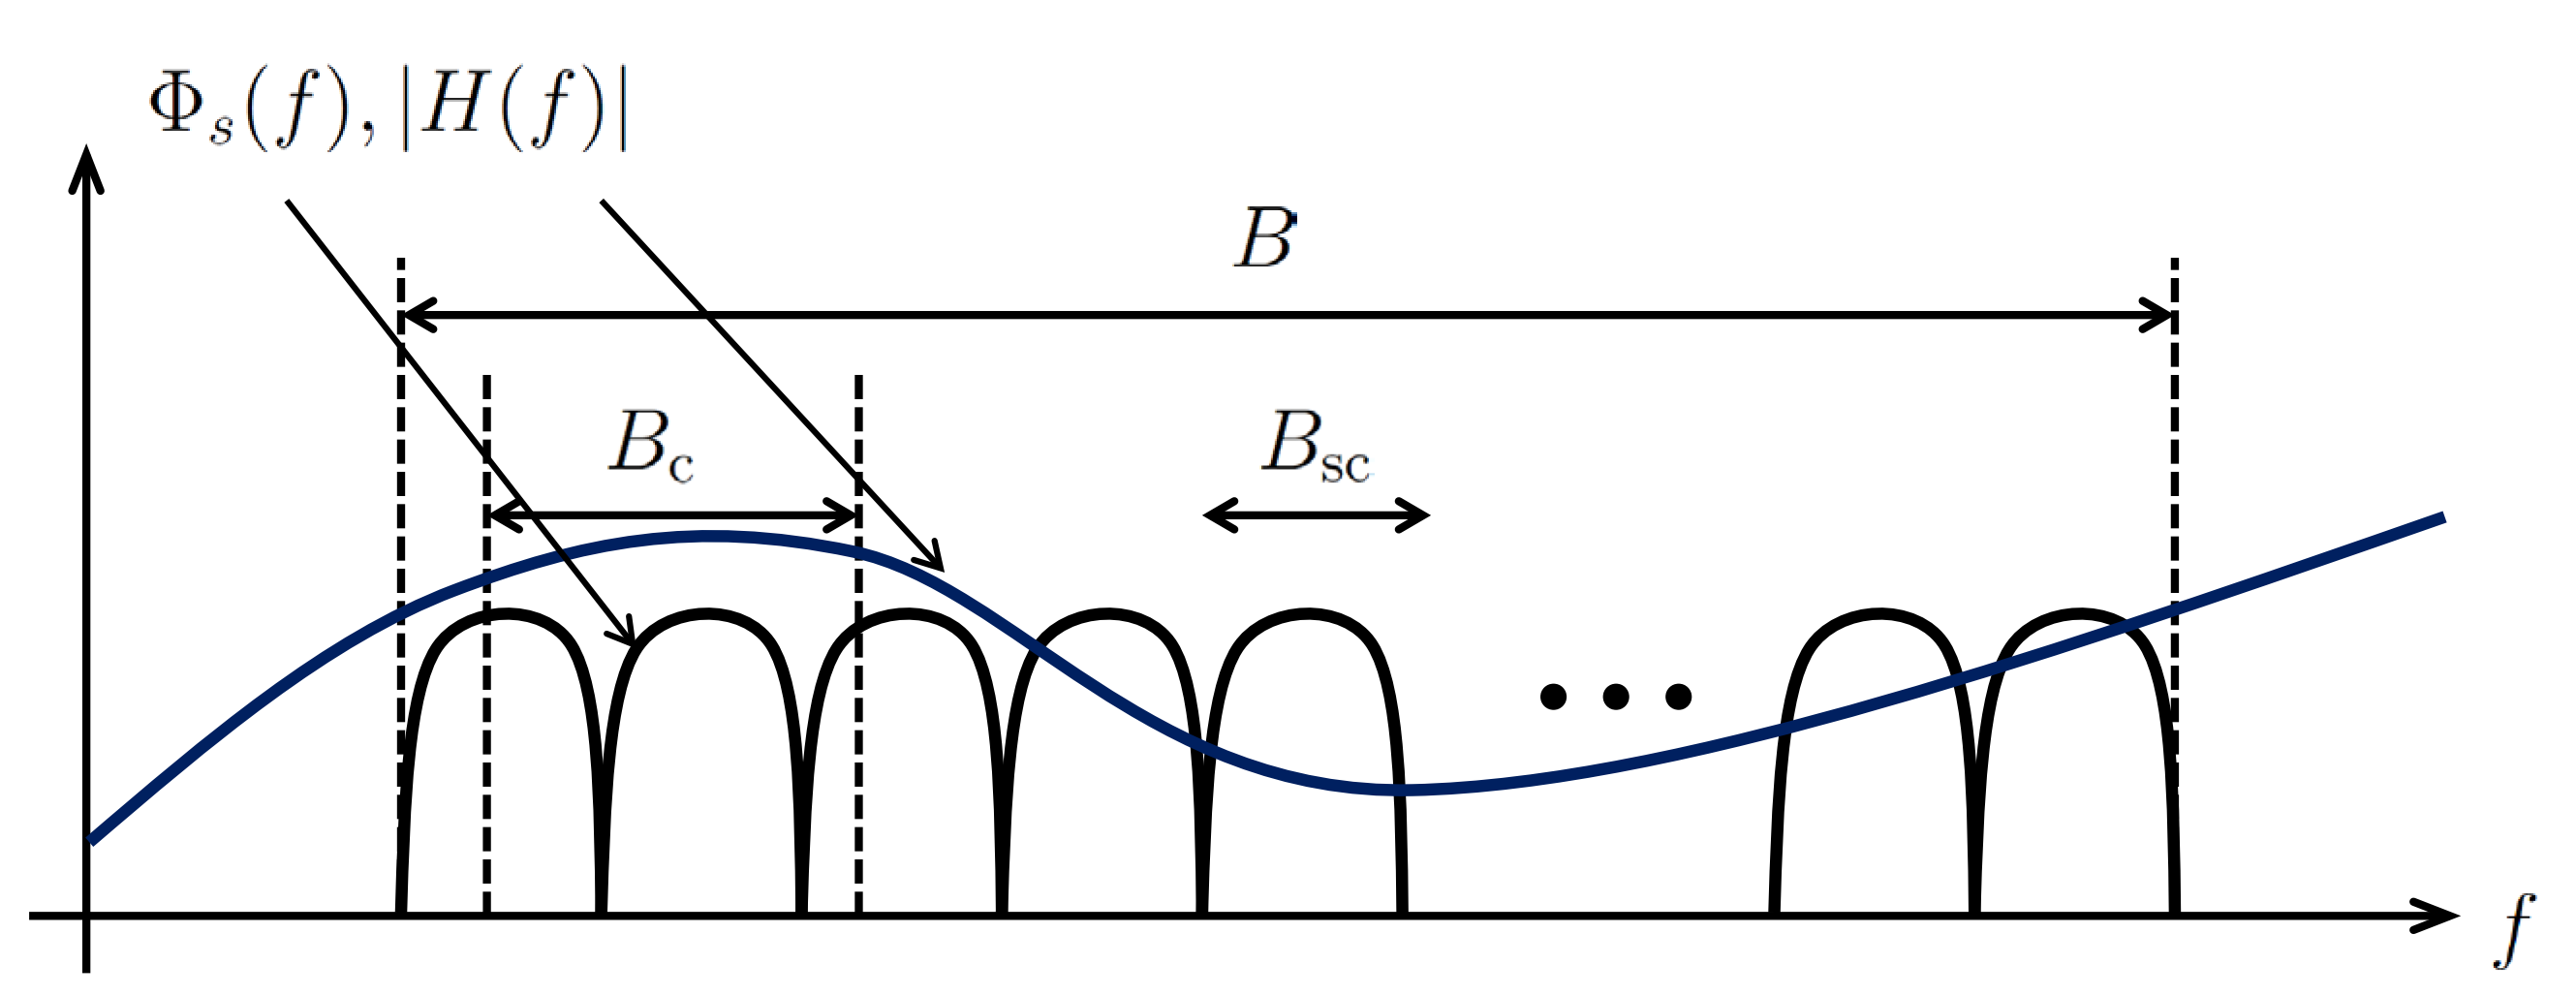
\includegraphics[width=.9\textwidth]{../fig/mehrtrager.png}
\end{center}

\section{OFDM}
Dauer des Kernsymbols: $T_{FFT}$ \\
Dauer des Schutzintervalls: $T_{cp}$ \\
Bedingung für interferenzfreien Empfang: $T_{cp} \geq \tau_m$
\begin{center}
	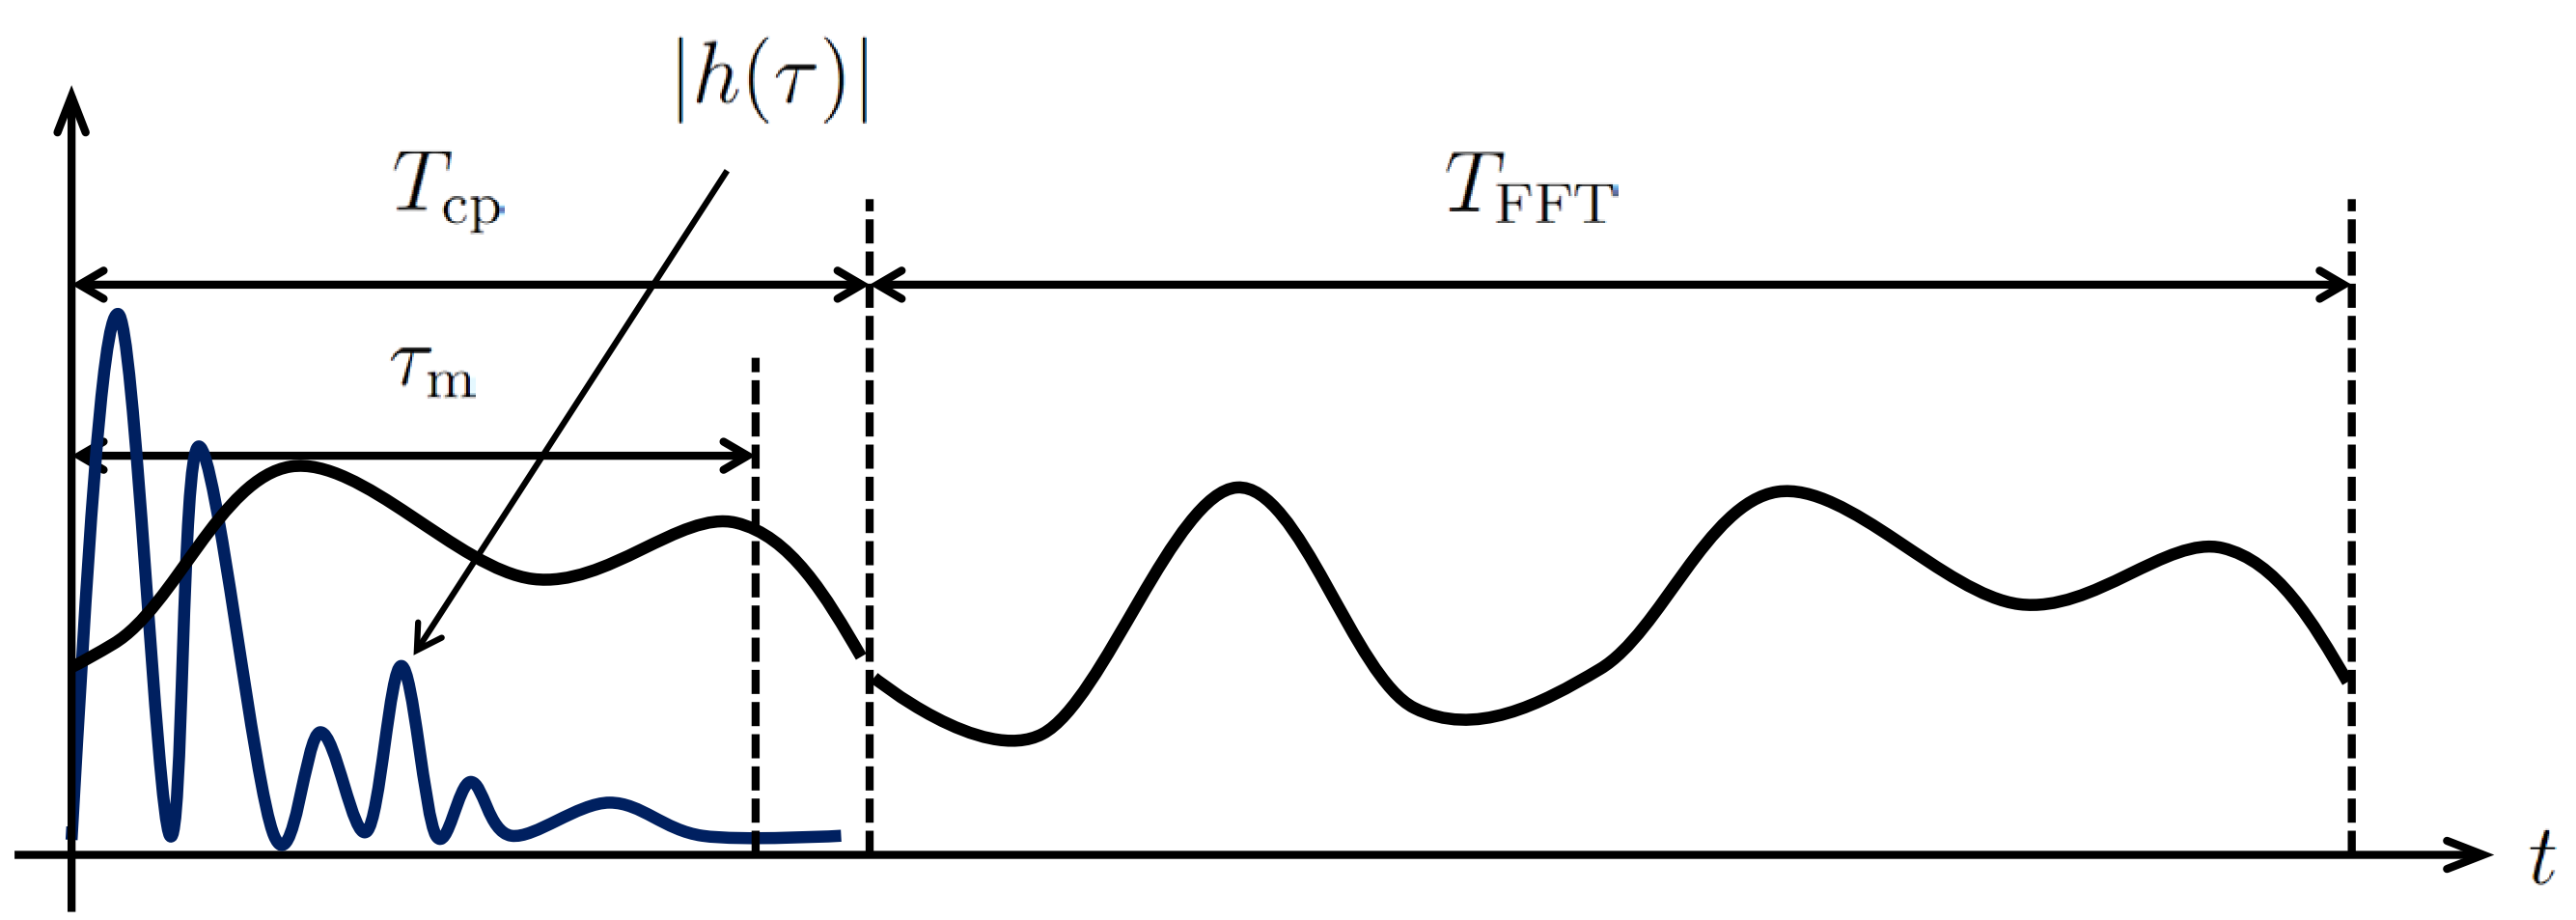
\includegraphics[width=.9\textwidth]{../fig/ofdm.png}
\end{center}
~\\
Bandbreite: $B$ \\
Unterträger: $K$ \\
Bandbreite Unterträger:
\[
	F = \frac{B}{K}
\]
~\\
Dauer des Kernsymbols:
\[
	T_{FFT} = \frac{1}{F}
\]
~\\
Dauer des Schutzintervalls:
\[
	T_{cp} \geq \frac{\textrm{längster Pfad [m]}}{3\cdot 10^8 \frac{m}{s}}
\]
~\\
Gesamtdauer:
\[
	T_{OFDM} = T_{cp} + T_{FFT}
\]
~\\
Bitrate:
\[ 
	R_b = \frac{K \cdot \textrm{Bit pro Symbol}}{T_{OFDM}}
\]
Spektrale Effizienz:
\[
	R/W = \frac{R_b}{B}
\]
